\documentclass{article}
\usepackage[utf8]{inputenc}
\usepackage[portuges]{babel}
\usepackage{listings}
\usepackage{xcolor}
\usepackage{verbatim}
\usepackage{indentfirst}
\usepackage{hyperref}
\setlength{\parindent}{6ex}
\usepackage{graphicx}
\usepackage{fancyhdr}
\usepackage{float}

\title{
       \vspace{60px}
       \Huge \textbf{Reverse Proxy} \\[15px]
       \Large \textbf{Relatório do trabalho prático}
       \vspace{100px}
      }
\author{
        \begin{tabular}{c}
            \textbf{Grupo 35} \\[5px]
                Ana Paula Carvalho (A61855) \\
                João Pires Barreira (A73831) \\
                Simão Barbosa (AXXXXX)
        \end{tabular}
       }
\date{Março 2018}

\makeatletter         
\def\@maketitle{
    \begin{center}
        \huge \@title \\[4ex]
        \Large \@author \\[5ex] 
        \@date \\[8px]
        \vspace{100px}
        
\includegraphics[scale=0.40]{img/uminho.png} \\
        \vspace{25px} 
        \small Comunicações por Computador \\[3px]
        Mestrado Integrado em Engenharia Informática \\[3px]
        Universidade do Minho \\
    \end{center}}
\makeatother

\begin{document}
\maketitle

\newpage
\section{Introdução}

Este projeto surge no âmbito da Unidade Curricular de Comunicações por Computador e tem como objetivo a implementação de um proxy reverso com balanceamento de carga.

O servidor \emph{proxy} deverá guardar informação acerca dos servidores de \emph{back-end} disponíveis e, sempre que chegar um pedido TCP vindo de um clinte, deve escolher o servidor mais apropriado para essa ligação (i.e. com menos carga a nível de RTT, CPU e RAM disponíveis, etc.).

\section{Arquitetura da solução}

A arquitetura da solução implementada encontra-se descrita na figura apresentada abaixo:

\begin{figure}[H]
    \centering
    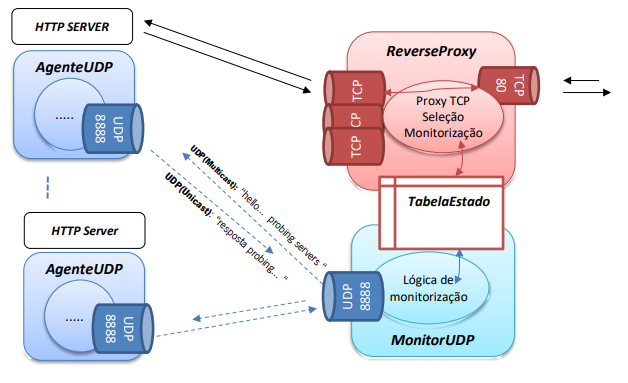
\includegraphics[scale=0.7]{img/arquitetura.PNG}
    \caption{Arquitetura da solução implementada}
\end{figure}

O servidor proxy guarda informação relativa

Resumidamente, são enviados pedidos HTTP para a porta 80 do servidor de \emph{proxy} que mantém informação acerca do estado dos servidores de \emph{back-end} numa tabela de decisão. Ao receber cada um destes pedidos via \emph{TCP}, o servidor \emph{proxy} escolhe o melhor servidor de \emph{back-end} disponível para o atender. Depois, o \emph{proxy} atua como um mero intermediário, encaminhando a informação recebida do cliente para o servidor e vice-versa.

Paralelamente a isto, a comunicação entre servidor \emph{proxy} e servidores de \emph{back-end} é feita através de \emph{UDP} através dos seguintes componentes:

\begin{itemize}
    \item \textbf{MonitorUDP}: Sendo responsável pela descoberta de servidores, de t em t segundos envia uma mensagem de probing por UDP (encriptada usando \emph{SHA-256}), dirigida ao grupo Multicast 239.8.8.8 para a porta 8888; depois, escuta as respostas UDP unicast na mesma porta, verificando a integridade de todas as mensagens recebidas (encriptadas usando \emph{SHA-256}) antes de atualizar a tabela de estado em conformidade
    \item \textbf{AgenteUDP}: Existindo um agente por cada servidor de \emph{back-end}, estes ficam à escuta de pedidos de probing (encriptados) na porta 8888 enviados pelo MonitorUDP por multicast para o grupo com endereço IPv4 239.8.8.8 (juntando-se previamente a este grupo). Por cada mensagem recebida, o AgenteUDP deve responder com uma mensagem encriptada UDP dirigida em unicast ao MonitorUDP, incluindo na resposta a carga da máquina (RAM e CPU). As respostas são artificialmente atrasadas, por um pequeno intervalo de tempo aleatório entre 0 e 10 ms, de modo a não serem enviadas todas ao mesmo tempo.
\end{itemize}

\section{Especificação do protocolo UDP}

O protocolo desenvolvido para a comunicação entre o MonitorUDP (do \emph{proxy}) e os AgentesUDP (dos servidores de \emph{back-end}), foi implementado, a nível aplicacional, com recurso ao UDP.

\subsection{Formato das mensagens protocolares}

\subsubsection{Formato da mensagem de probing (ProbeRequest)}

\begin{itemize}
    \item \textbf{timestamp} -- campo do tipo \emph{long} que serve para denotar a marca temporal relativa ao momento em que foi enviado a mensagem de ProbeRequest (será utilizado para cálculo do RTT).
    \item \textbf{hmac} -- campo que possui o output gerado pela encriptação da mensagem de ProbeRequest com recurso ao SHA-256.
\end{itemize}

Assim sendo, cada mensagem de ProbeRequest tem um \textbf{tamanho fixo de 40 bytes}, correspondentes aos 8 bytes do timestamp e 32 bytes (256 bits) do HMAC gerado pelo SHA-256.

\subsubsection{Formato da mensagem de resposta ao probing (ProbeResponse)}

\begin{itemize}
    \item \textbf{cpuUsage} -- byte que corresponde à percentagem de CPU que está ser utilizada pelo servidor de \emph{back-end}
    \item \textbf{freeRAM} -- 4 bytes que correspondem à quantidade de RAM disponível no servidor de \emph{back-end} (em megabytes)
    \item \textbf{timestamp} -- campo do tipo \emph{long} que serve para denotar a marca temporal relativa ao momento em que foi enviado a mensagem de ProbeRequest (será utilizado para cálculo do RTT).
    \item \textbf{hmac} -- campo que possui o output gerado pela encriptação da mensagem de ProbeRequest com recurso ao SHA-256.
\end{itemize}

Assim sendo, cada mensagem de ProbeResponse tem um \textbf{tamanho fixo de 45 bytes}, correspondentes aos 4 bytes de freeRam, 1 bytes de cpuUsage, 8 bytes do timestamp e 32 bytes (256 bits) do HMAC gerado pelo SHA-256.

\subsection{Interações}

As interações entre o MonitorUDP e os AgentesUDP encontram-se explicadas nos dois pontos da parte inferior da secção \textbf{Arquitetura da solução}.

No entanto, é importante explicitar melhor a encriptação das mensagens envidas e recebidas. Para isto, foi utilizado o algortimo de hash chamado \emph{SHA-256} por ser um algoritmo seguro e robusto. Desta forma, tanto o MonitorUDP como os AgentesUDP possuem uma chave privada partilhada entre ambos. Antes de enviarem uma mensagem, pegam nos conteúdos dessa mensagem e, como eles, geram um byte array correspondente ao HMAC gerado pela chamada do algortimo SHA-256 com a combinação desses mesmo conteúdos e da chave privada. Assim, o recetor ao receber a mensagem, vai fazer o mesmo analogamente, gerando um código que depois terá de ser comparado ao recebido. Como, ambos partilham a mesma chave privada e os conteúdos são os mesmo, irão obter o mesmo código HMAC, pelo que fica assegurada a autenticidade da origem visto que sem aquela chave privada não seria possível gerar o mesmo output, pela definição da função de hash.

\section{Implementação}

Para a implementação destes conceitos, foi utilizada a linguagem de programação orientada a objetivos \emph{Java}, e definidas as seguintes classes:

\begin{itemize}
    \item \textbf{HMAC} - Implementa as funcionalidade referidas na subsecção \textbf{Interações}.
    \item \textbf{ProbeRequest} - Implementa as funcionalidade referidas na subsecção \textbf{Formato da mensagem de probing}.
    \item \textbf{ProbeResponse} - Implementa as funcionalidade referidas na subsecção \textbf{Formato da mensagem de resposta ao probing}.
    \item \textbf{UDPMonitor} - Implementa as funcionalidade referidas na descrição deste componente na secção \textbf{Arquitetura da solução}. Para isso, foi criada uma função main que lança uma thread de probing que envia pedidos de probing encriptados através de Multicast UDP. Paralelamente, para cada resposta recebida em unicast, é lançada outra thread responsável por verificar a integridade da resposta e atualizar a tabela de estado. É feito \emph{logging} do envio e receção de mensagens para o standard output.
    \item \textbf{UDPAgent} - Implementa as funcionalidade referidas na descrição deste componente na secção \textbf{Arquitetura da solução}. Para isso, foi criada uma função main que, em primeiro lugar, se junta ao grupo Multicast (UDP), ficando à espera de um pedido de probing enviado pelo MonitorUDP. Assim que recebe uma resposta, verifica a integridade da mensagem recebida e, caso esta seja verficada com sucesso, lança uma thread responsável por retirar as medidas necessárias do servidor \emph{back-end} associado (CPU e RAM), encriptar a resposta e, de seguida, enviar a mesma por unicast UDP ao MonitorUDP, atrasando artifialmente este envio por um período aleatório entre 1 e 10 segundos. É feito \emph{logging} do envio e receção de mensagens para o standard output.
    \item \textbf{ServeStatus} - Possui as informações relativas ao estado de um servidor de \emph{back-end}, nomeadamente: o endereço IP, a porta, o timestamp do última resposta de probing recebida, a RAM disponível, o CPU a ser utilizado, o RTT atual, o somatório de todos os RTT até ao momento e o número de respostas recebidas. Estes dois últimos campos servem para calcular o RTT atual através da média.
    \item \textbf{StatusTable} - Tabela de estado que é atualizada pelo MonitorUDP do ReverseProxy e que contém a informação acerca dos estados (ServerStatus) de todos os servidores de \emph{back-end}. A função de update, verifica se a informação recebida é mais recente do que a que já constava da tabela e, em caso afirmativo, calcula o RTT do percurso (através do timestamp da PDU e do tempo atual). É necessário fazer-se um controlo de concorrência ao nível desta tabela, por causa das diferentes threads que estão a correr (MonitorUDP) que podem despoletar updates simultaneos. A função chooseServer é a responsável por escolher o servidor com melhores condições atuais, através de uma heurística simples que atribui um peso definido pelo grupo para cada uma das medidas de estado do servidor.
    \item \textbf{ReverseProxy} - É a classe principal do programa. A sua função main inicia a estrutura de dados relativa à tabela de estado e coloca o MonitorUDP a correr. Paralelamente, cria os sockets para a comunicação com o cliente e com o servidor de \emph{back-end} que será escolhido através da função chooseServer da StatusTable sempre que é recebido um pedido HTTP de um cliente. A comunicação enter servidor e cliente é reencaminhada pelo proxy de forma transparente e direta.
\end{itemize}

\newpage
\section{Testes e resultados}

Para efeitos de teste foi utilizado o software \emph{CORE} com a topologia fornecida durante as aulas que se encontra representada na imagem seguinte:

\begin{figure}[H]
    \centering
    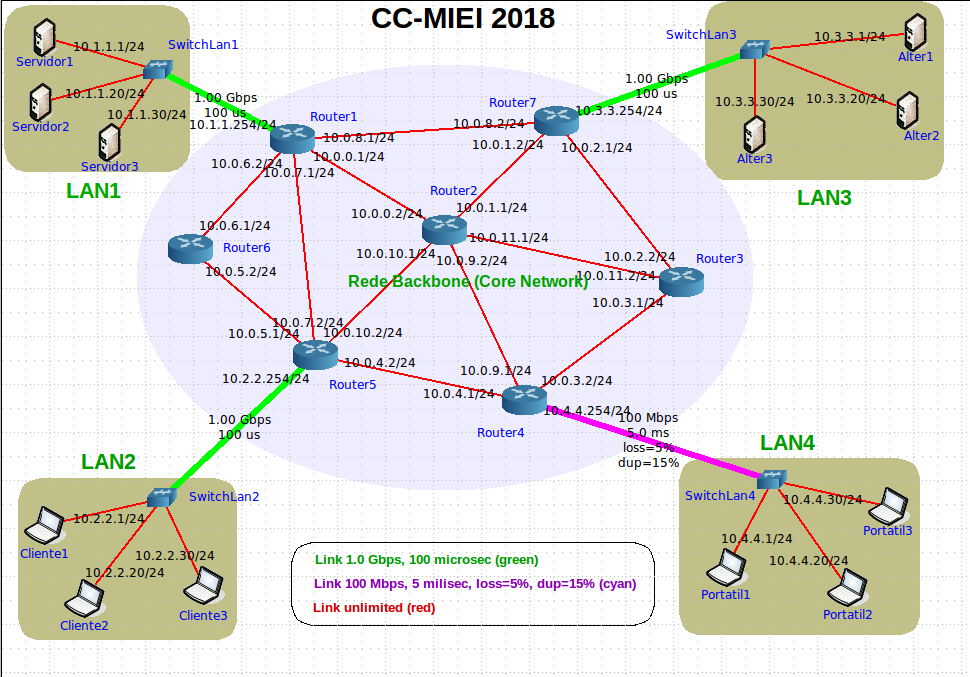
\includegraphics[scale=0.3]{img/topologia.png}
    \caption{Topologia CORE utilizada}
\end{figure}

Desta forma, foi posto a correr no Servidor 1 o ReverseProxy; em cada um dos Servidores 2 e 3 foi posto a correr um servidor HTTP simples feito em Python 3 (SimpleHTTPServer) e um AgenteUDP. Esta situação está descrita na seguinte imagem:

\begin{figure}[H]
    \centering
    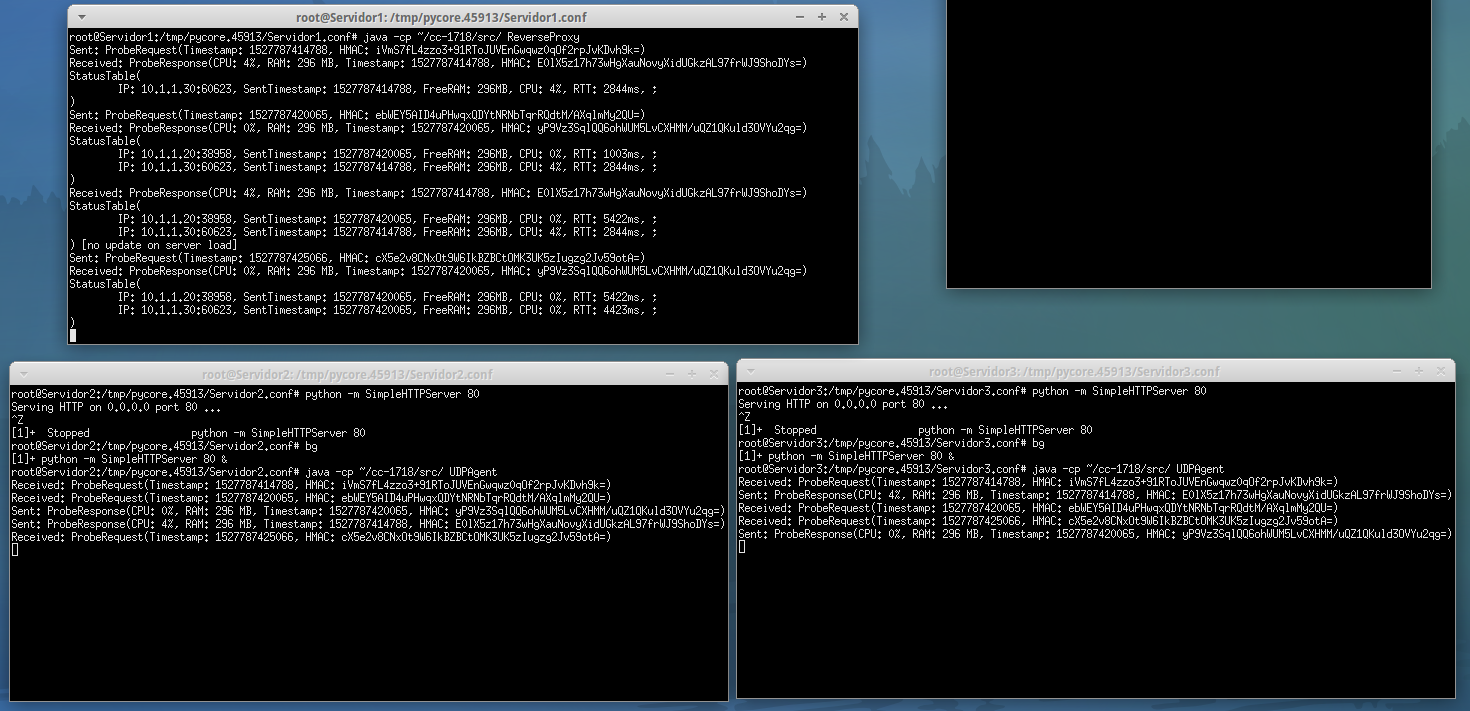
\includegraphics[scale=0.3]{img/semcliente2.png}
    \caption{Servidor 1 (ReverseProxy) e Servidor 2 e Servidor 3 (AgentesUDP com servidor HTTP)}
\end{figure}

Como podemos verificar, o ReverseProxy e os AgentesUDP encontram-se a correr corretamente e a trocar mensagems (pedidos e respostas de probing entre si). Além disso, é imprimida tambéma a tabela de estado e caso não haja atualização da tabela após uma resposta recebida por esta conter informação mais antiga do que a que já constava na tabela, aparece uma marca "no update on server load".

No portátil 1, pusemos a correr um cliente que faz a conexão ao ReverseProxy, sendo-lhe enviada a resposta contendo um ficheiro index.html. De notar, que no exemplo abaixo foi escolhido o servidor 2 para efetuar a conexão com o cliente por ter os melhores valores, nomeadamente o RTT (pode-se verificar isso abaixo, no log do Servidor 1, o proxy).

\begin{figure}[H]
    \centering
    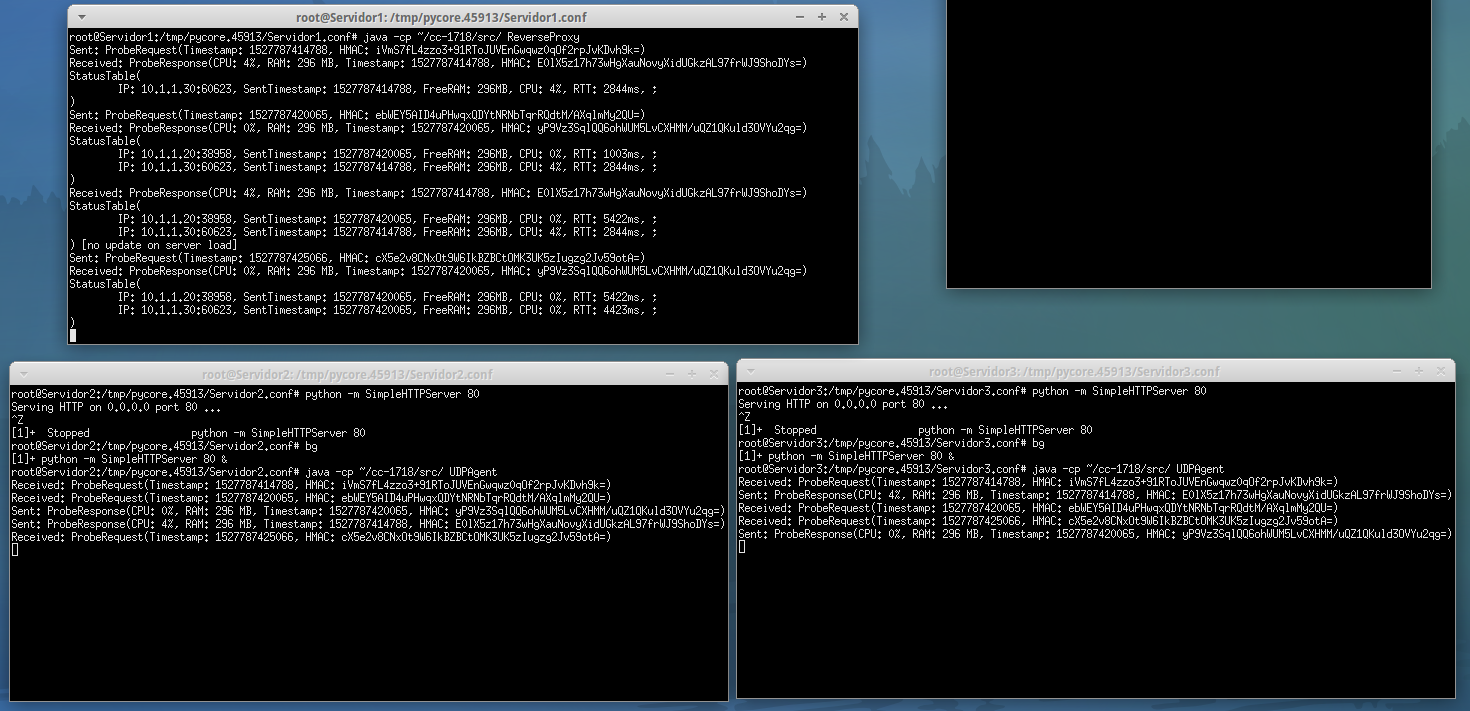
\includegraphics[scale=0.3]{img/semcliente2.png}
    \caption{Cliente (Portatil1) conectou-se com sucesso}
\end{figure}

\begin{figure}[H]
    \centering
    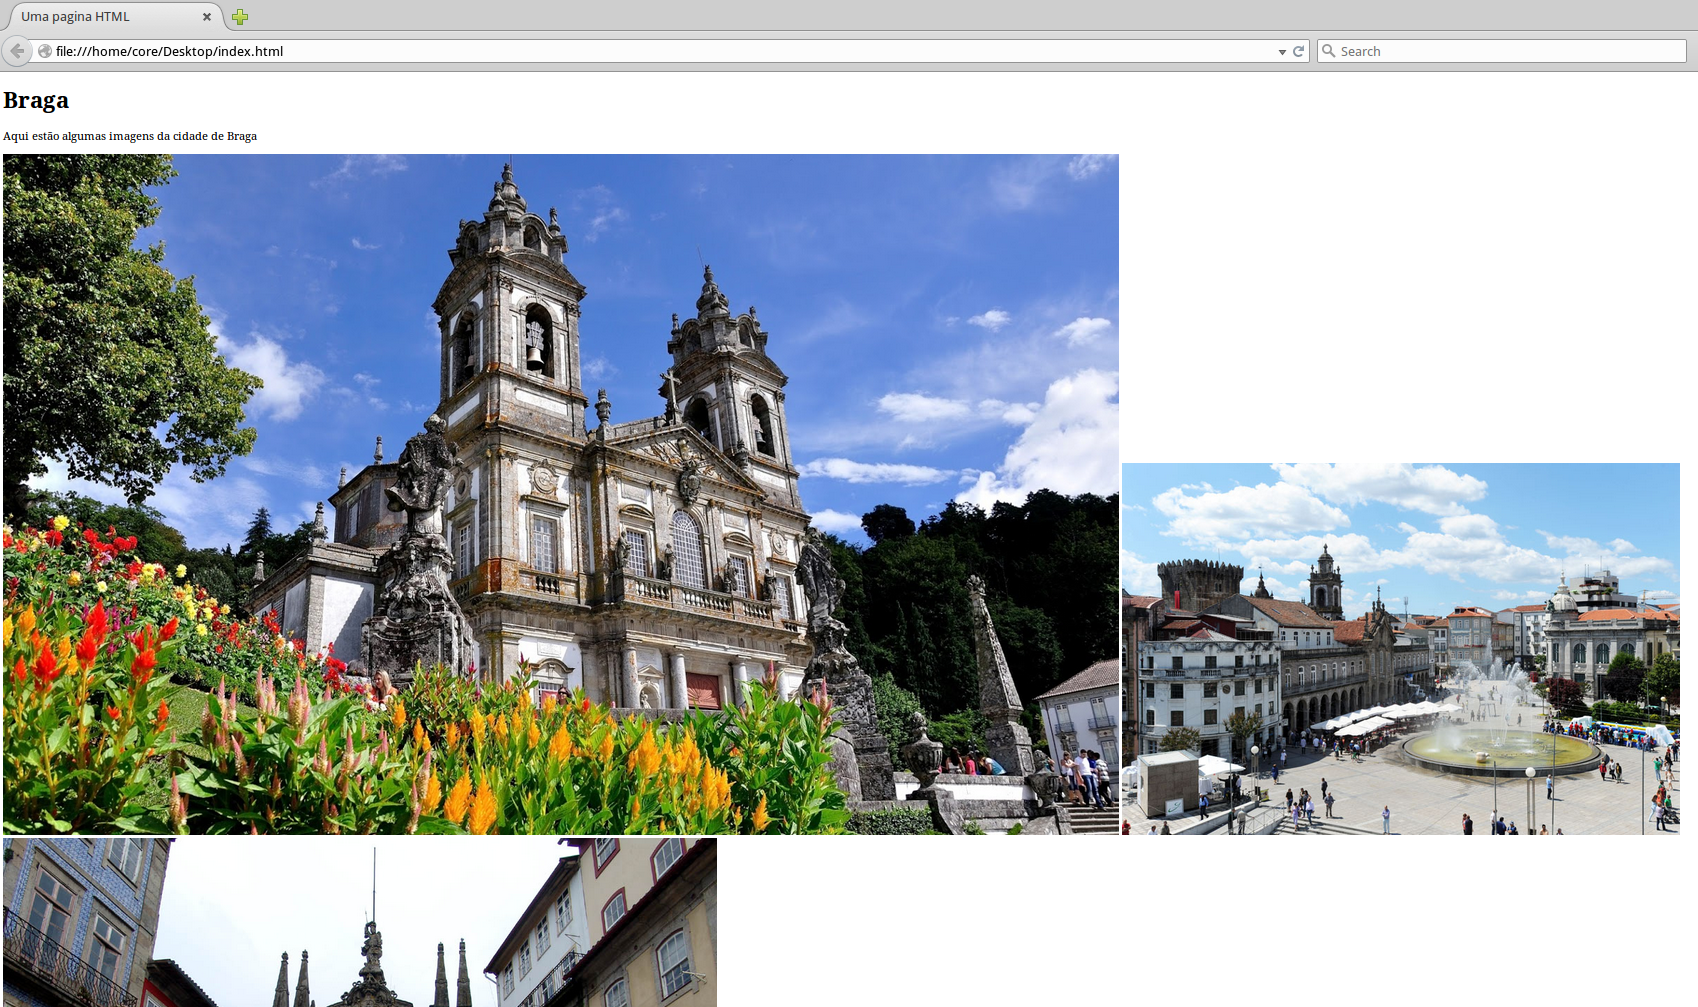
\includegraphics[scale=0.2]{img/site.png}
    \caption{Index.html recebido}
\end{figure}

\newpage
Num segundo exemplo, pusemos o cliente a tentar conectar-se não havendo ainda qualquer servidor de \emph{back-end} disponível. Assim, o cliente recebeu uma mensagem de erro HTTP 404 enviada pelo ReverseProxy (MonitorUDP), como se pode verificar pela imagem abaixo:

\begin{figure}[H]
    \centering
    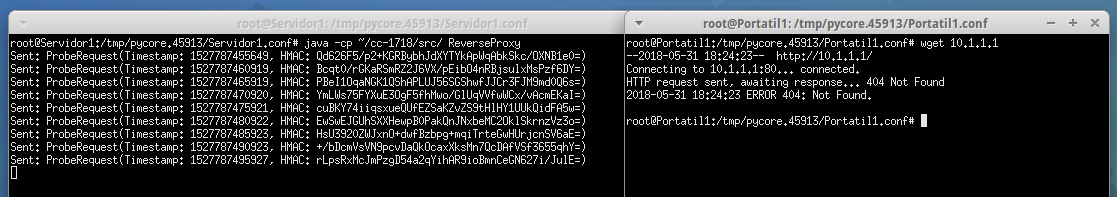
\includegraphics[scale=0.4]{img/noservers.png}
    \caption{Index.html recebido}
\end{figure}

\newpage

\section{Conclusões e trabalho futuro}

Após a conclusão deste projeto prático o grupo conseguiu implementar com sucesso o \emph{reverse proxy} proposto. Incluiram-se os componentes exigidos e as funcionalidades como os envios de mensagens de \emph{probing} e receção das respostas às mesmas, distinção entre envios em \emph{Multicast} e \emph{Unicast}, respostas quanto à carga da máquina, etc. 

Para trabalho futuro, visto que não houve a oportunidade de incorporar essa funcionalidade na nossa solução por escassez de tempo, poderia-se estruturar um tratamento para as quebras de conexões de servidores do \emph{back-end}.

Em suma, a realização deste trabalho proporcionou-nos uma destreza e um conhecimento mais completo quando aos conteúdos lecionados aos longo das aulas teóricas e práticas, revelando-se uma atividade vantajosa para alcançar um bom resultado na Unidade Curricular de Comunicações por Computador.

\end{document}
